\newpage
\section{Human FER during Speech}
\label{sec:human}
Given the limitations of automatically detecting emotion in speaking faces, we look at the human ability of categorizing affective state. Are humans more accurate than our existing models when confronted with talking subjects? Are there notable variations in their performance? Insights from the human perception of emotions on speaking subjects can help us create models that are more robust against speech. The CREMA-D corpus \cite{cao2014crema} includes aggregated results of the ratings collected from crowd-sourced labellers. These already give insights in human biases when categorizing emotion in talking subjects.

The videos in the CREMA-D corpus were acted and scripted. The actors were given a sentence and were tasked to speak that sentence in a given emotion. Annotators later evaluated these videos in three different modes:

\begin{enumerate}
    \item Audio only
    \item Video only
    \item Audio and Video
\end{enumerate}

We focus on the video-only task, since our models will also be only in the visual domain. Depending on the emotion, the annotators accuracy are significantly different. Videos on a happy emotion were labelled correctly 88\% of the time, whereas sad videos only had an accuracy of 32\% (Figure \ref{fig:crema_results}). The overall accuracy of the video-only annotation stands at 58.2\%.

\begin{figure}
    \centering
    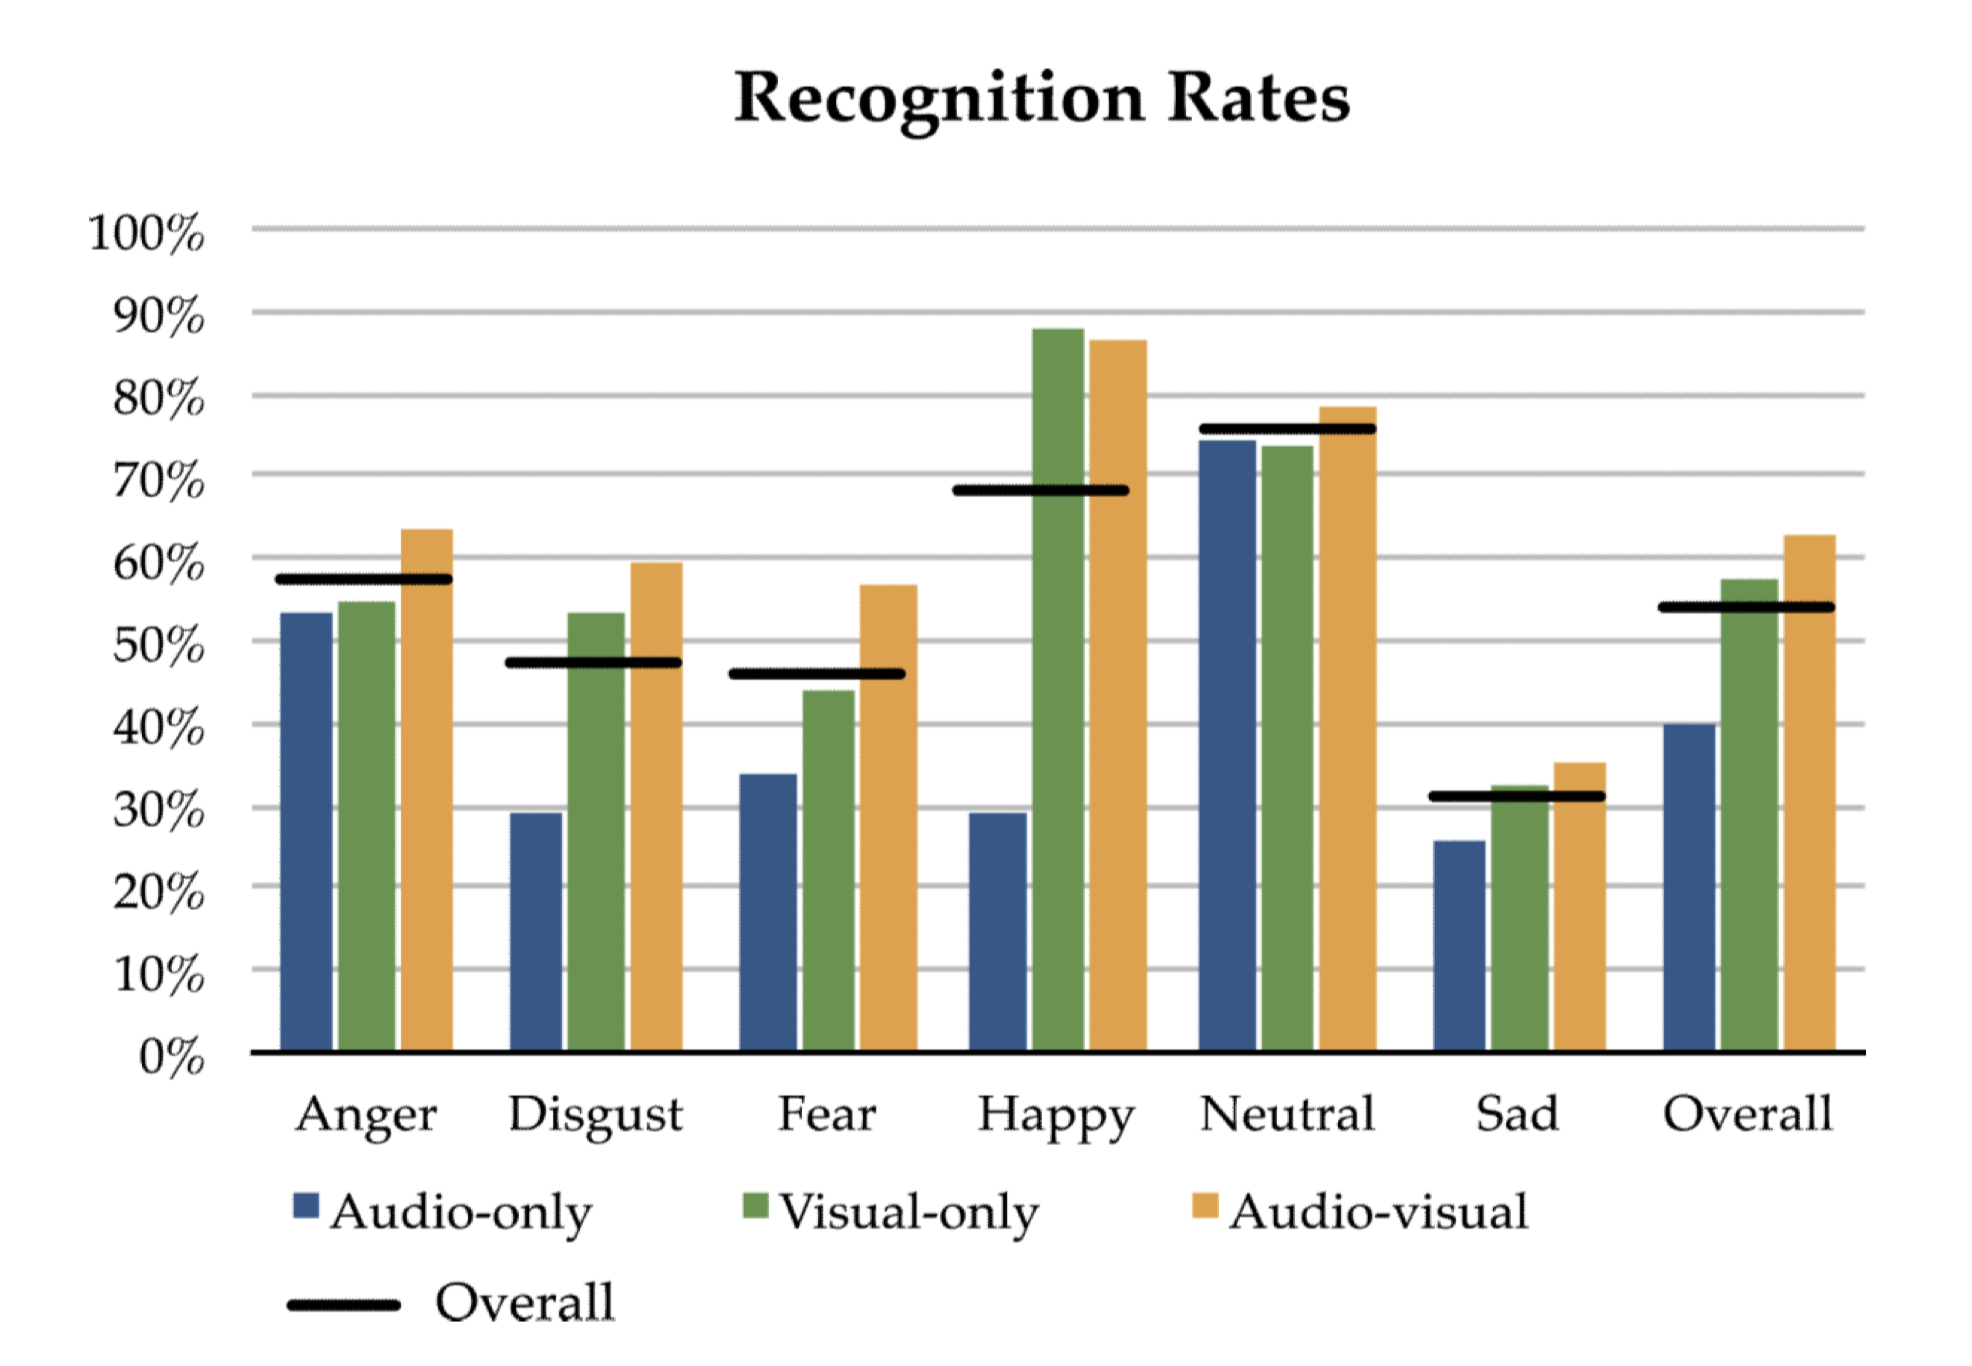
\includegraphics[width=0.8\textwidth]{res/crema.png}
    \caption{The results of the human annotation on the CREMA-D corpus \cite{cao2014crema}. There generally is a trend for audio-visual videos to be labelled better than visual-only data. There are also differences in accuracy depending on the emotion.}
    \label{fig:crema_results}
\end{figure}

Some questions remain unanswered. How do human annotators perform if they are confronted with still images of people talking? Are there any significant differences in accuracy depending on the phoneme that is spoken in the image? Those questions may help us in constructing a FER model that is robust against speech. 

We will first analyse the performance of existing FER models against speaking subjects. Since our classic FER models are trained on single images, we will use still frames to evaluate them. We then analyse the phonetic bias of the model (Figure \ref{fig:phone_acc_ravdess}). The accuracy of our model differs depending on the phoneme. The best phonemes \texttt{Z} and \texttt{IY0} have accuracies of 49\%, whereas the worst performing phoneme \texttt{AY1} has an accuracy of only 40\%.
%With the help of the MFA (Section \ref{sub:mfa}) we were able to extract frames from the RAVDESS database (Section \ref{sub:ravdess}) with their respective phoneme labels
\begin{figure}
    \centering
    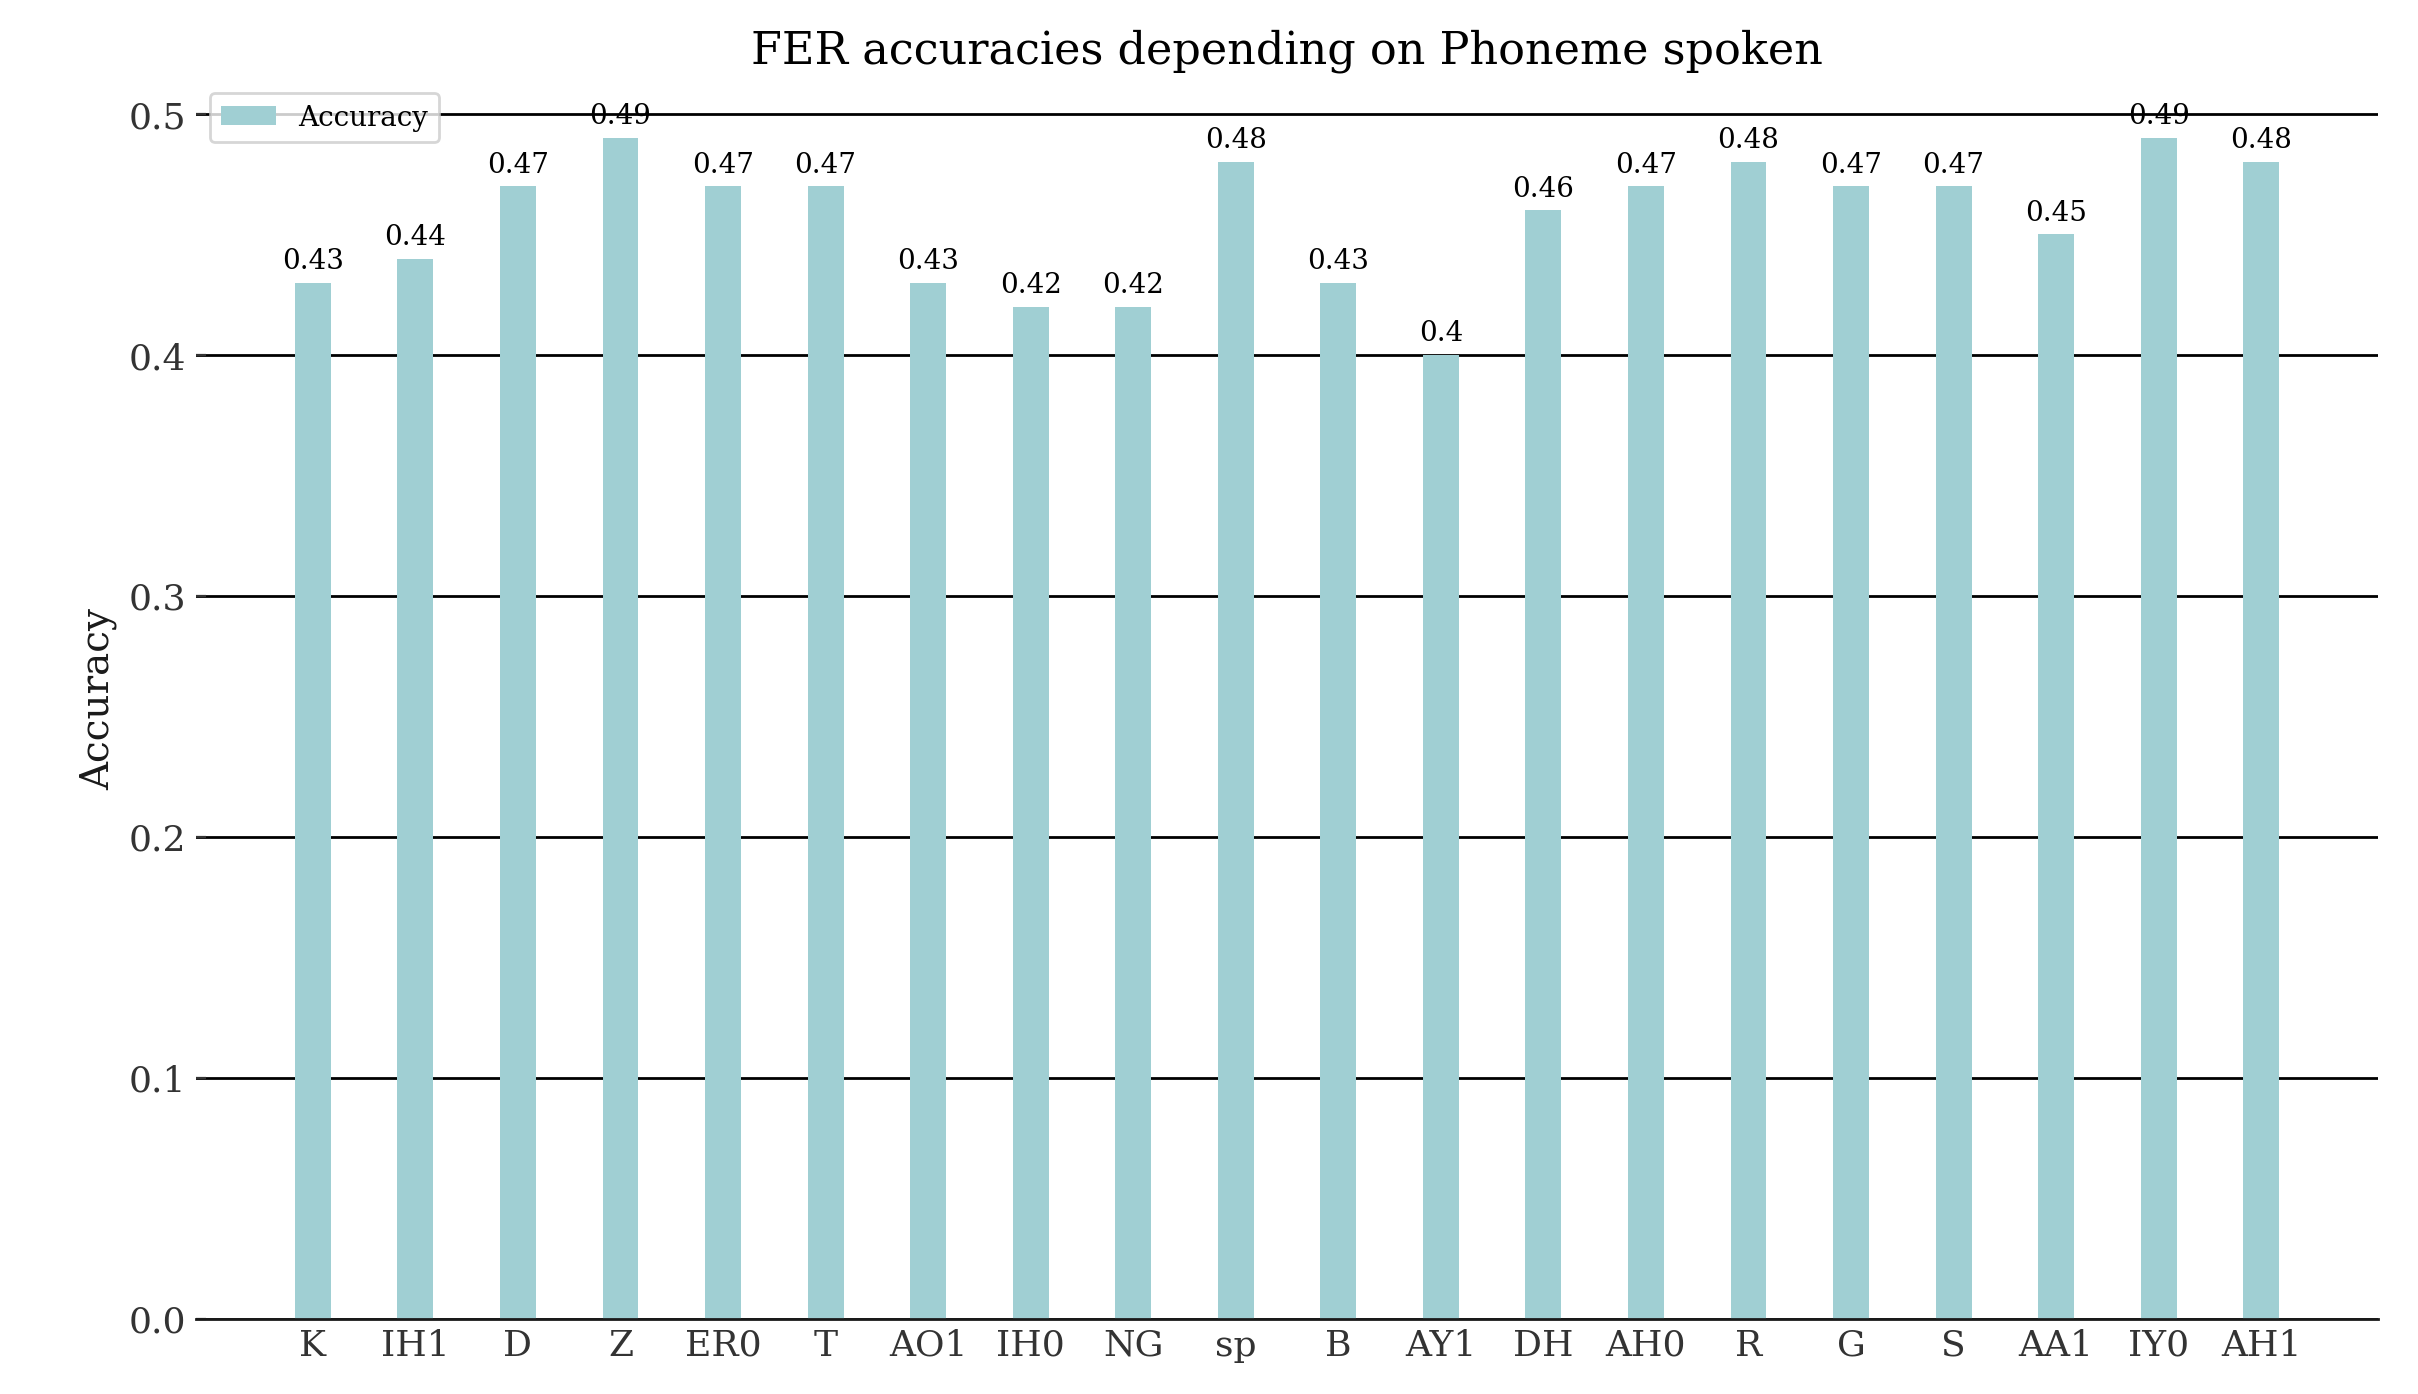
\includegraphics[width=0.8\textwidth]{res/FERvsPHONE.png}
    \caption{Accuracies of our classic FER model depending on the phoneme that was spoken in the classified frame. Accuracies range from 40\% to 49\%, showing a significant bias on the spoken phonemes.}
    \label{fig:phone_acc_ravdess}
\end{figure}
\subsection{Goal}
We have seen that our classic FER models perform differently depending on the phoneme. Human annotators have differing performance based on emotions. An analysis on human bias depending on phoneme is however missing. Getting insights into human performance on emotion estimation depending on the spoken phoneme can help us in our task to build FER models that are more robust towards speech.

Is human bias similar to the bias shown in our models? Are humans capable to judge the emotional state of a speaking subject just by looking at a single frame, or does the performance increase when a video (without sound) is available? These are the questions we want to answer in this section.

\subsection{Setup and Material}
We turned to the RAVDESS dataset \cite{livingstone2018ryerson} for the material of our study. Compared to the CREMA-D corpus, RAVDESS also includes the \texttt{surprised} emotion, which will be part of our future models. We want our annotators to label the videos and selected still images from those videos. Given the size of the RAVDESS corpus, we decided to label a subset of the database. Videos of actors 4 (f), 5 (m), 9 (m), and 14 (f) were chosen, with two videos for each of the seven core emotions. The \texttt{calm} emotion was ignored, because it will not be part of our future models since they will follow the seven core emotions from Ekman. This amounts to $4 \cdot 7 \cdot 2 = 56$ videos. To keep the amount of image labels manageable, we chose a subset of phonemes. Our choices were the phonemes \texttt{AY1}, \texttt{Z}, and \texttt{B}. We chose those phonemes because they include some of the best and worst performing phonemes on the model. That way we can later compare the performance of human labellers on those phonemes and draw conclusions on human bias. The total amount of images was 168, with each phoneme being represented 56 times.

To limit faulty annotations due to fatigue at the end of a long labelling session, the data was split into two groups. The first group was labelling videos and images from actors 4 and 5 (Group 0405), and the second group was tasked with the data from actors 9 and 14 (Group 0914). In total, each group had to label 28 videos and 84 images.

Annotators were first labelled the images before continuing to the videos. Since the images were sourced from the same videos that were labelled we wanted to make sure that there was no bias on the image labels from the perception of the videos.
% This was done to make sure that the labels for the images were not biased by the perception of the videos.

The images and videos were stored in the firebase storage. Images and videos also had a respective collection in the Firestore database, where each file had a corresponding document with its meta data:

\begin{lstlisting}
{
    actor
    emotion
    fileName
}
\end{lstlisting}

Each group of batches also had a Firestore document in its \texttt{groups} collection, where the list of its videos and images were stored. A \texttt{meta} document stored the amount of batches labelled, which also determined the group of the next batch (even -> Group 0405, odd -> Group 0914).

\subsection{Implementation}
The study was done through a simple web application. It was implemented using Svelte for the frontend application (Figure \ref{fig:tool_screenshot}), while the data management and hosting was done through firebase. The annotations were saved in real-time, making sure that all completed labels were available in case of connection issues \cite{baur2021}.

Each batch was saved as a document in the Firestore Database. The document included the start time for labelling, the labelled group, a unique identifier, and the image and video selections in two separate dictionaries: 
% https://www.overleaf.com/learn/latex/Code_listing#Reference_guide

\begin{lstlisting}
{
    createdAt
    group
    id
    imageSelections: {
        imageId: label
    }
    videoSelections: {
        videoId: label
    }
}
\end{lstlisting}

\begin{figure}
    \centering
    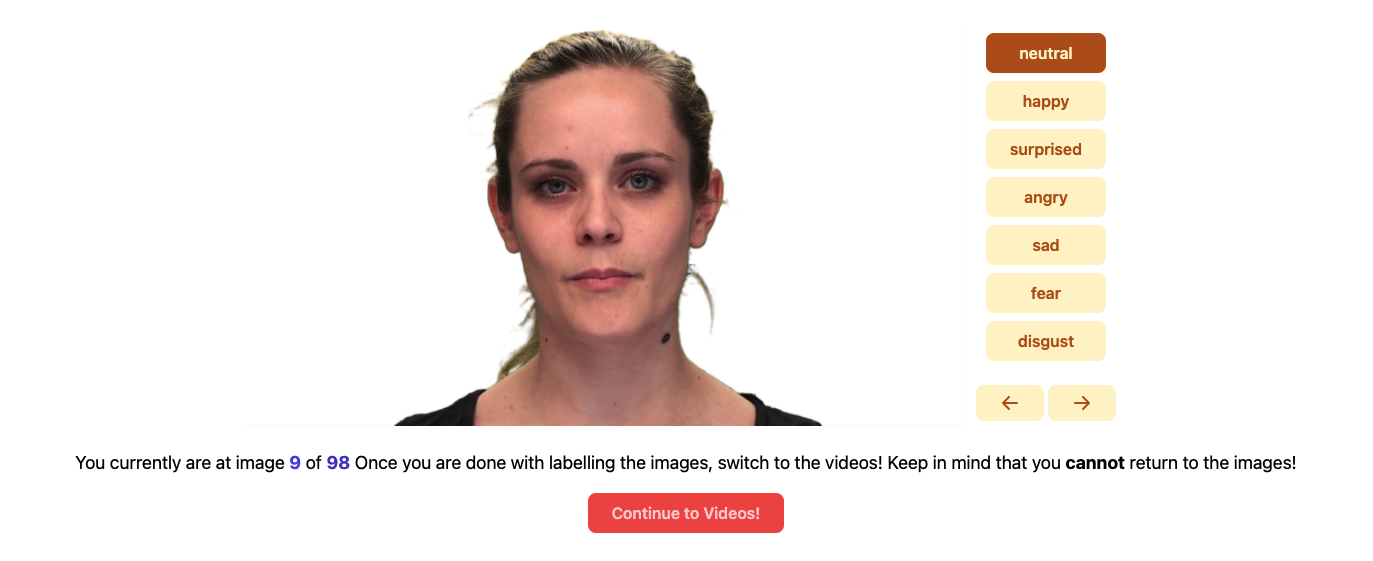
\includegraphics[width=0.8\textwidth]{res/LabellingTool.png}
    \caption{Screenshot from the labelling tool. The annotator is currently in the process of labelling the images, and has selected the \texttt{neutral} emotion for the current image.}
    \label{fig:tool_screenshot}
\end{figure}

\subsection{Annotators}
The annotators were recruited through personal contacts and a university seminar on a voluntary basis. In total, 16 participants annotated their batches. This leads to each data group being annotated eight times. All annotators were university students in their 20s.

Participants were prepared for the task through a presentation. They were especially told not to take too much time on each datapoint, to make sure that their first impression was determining the respective label.

\subsection{Discussion}
In this subsection we present and discuss the results of human labelling, and draw conclusions that can help us in building a FER model that is robust against speaking subjects.

\subsubsection{Temporal Dimension}
The annotators labelled both image and video data. The images are still frames from the videos. This allows us to compare the labelling performance between still frames and videos, and thus judge the importance of a temporal dimension. Our results, as seen in Figure \ref{fig:setting_overview}, conclude that 75.8\% of videos were labelled correctly, whereas the accuracy on the images was only 60.5\% (446 video labels, 1425 image labels). This indicates that temporal data may play an important role for FER when the subject is talking.


\begin{figure}
    \centering
    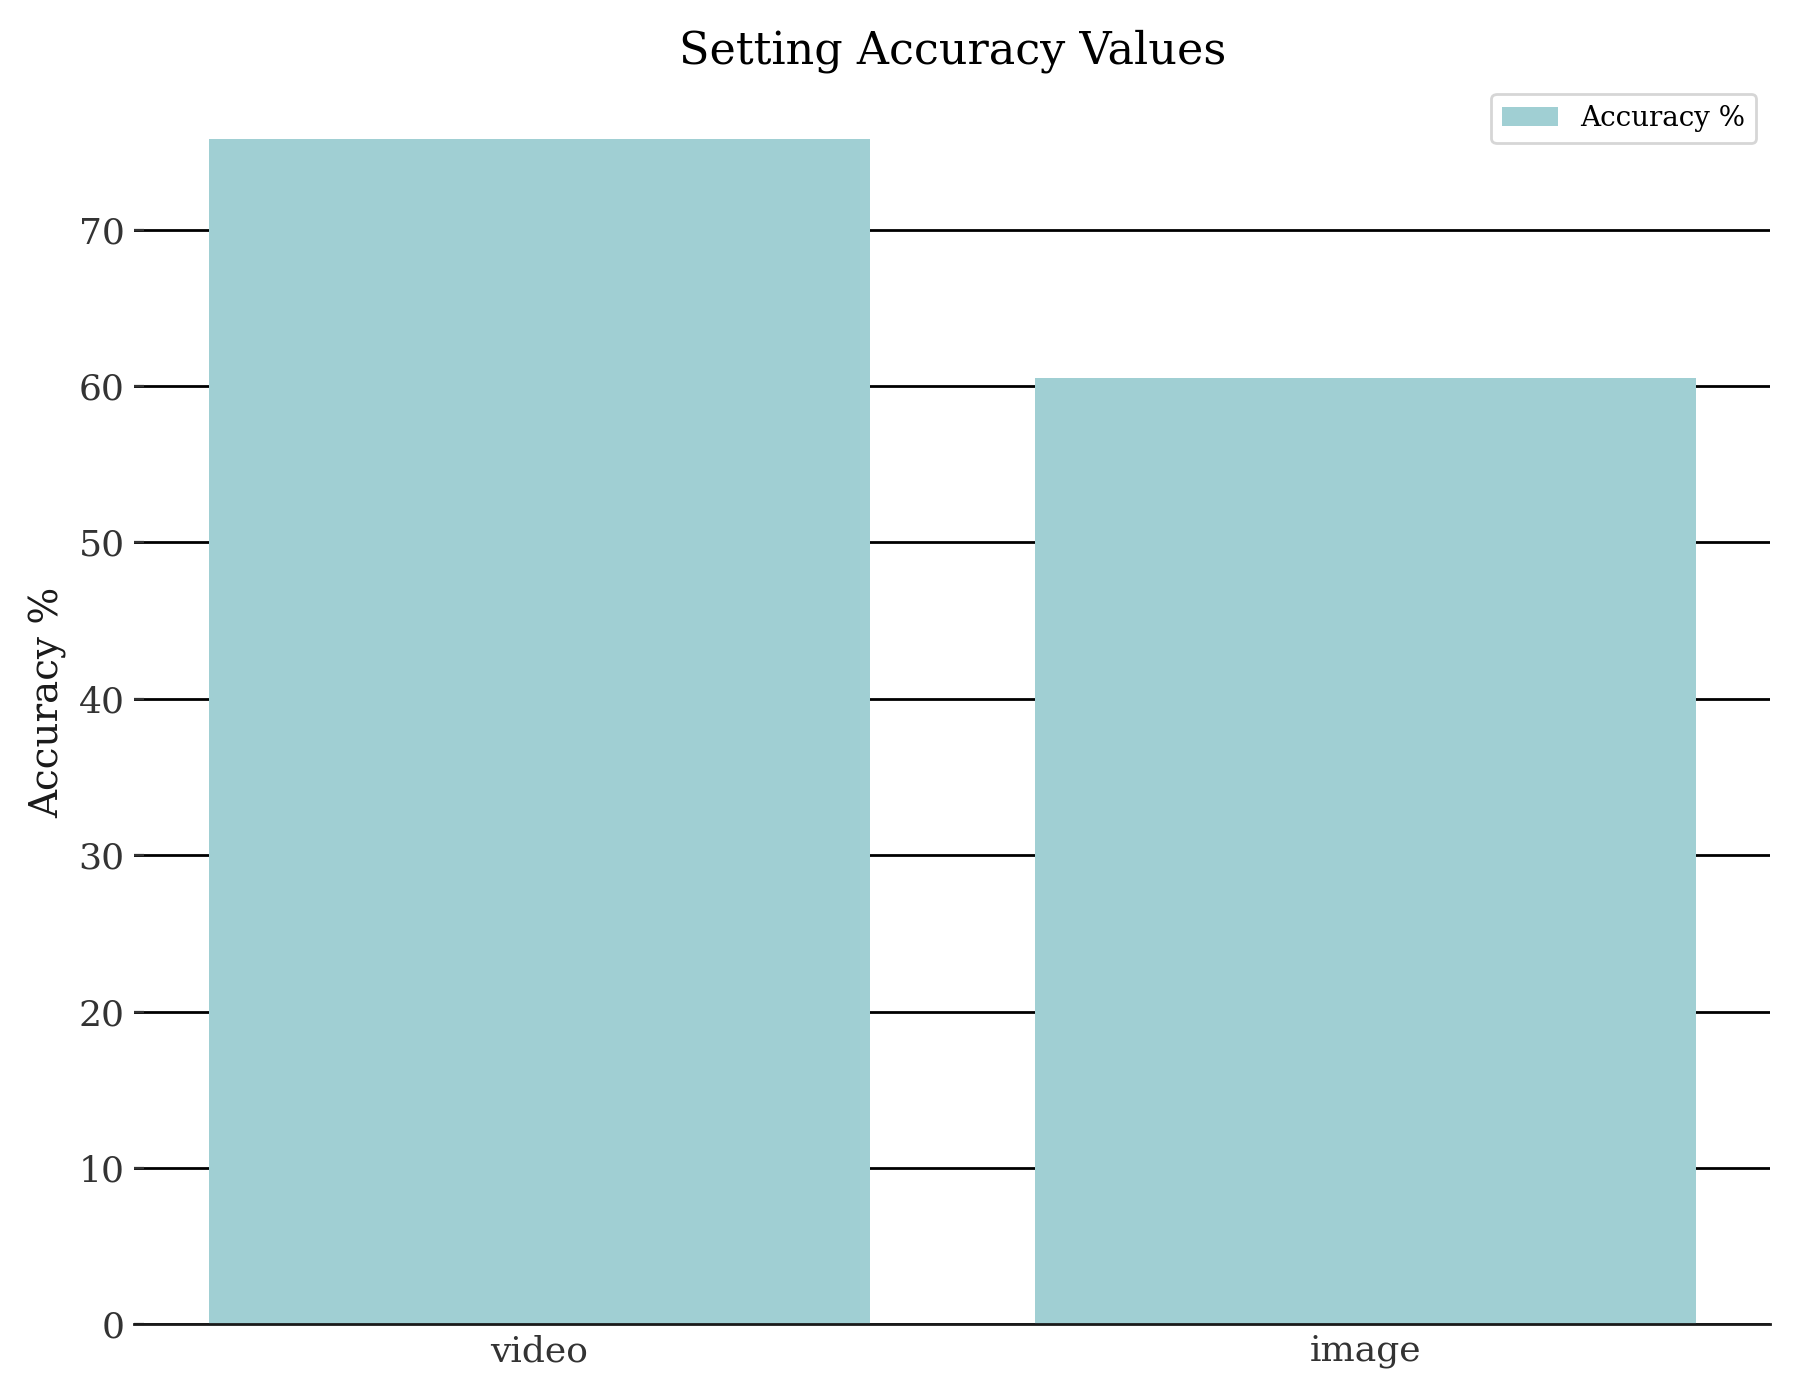
\includegraphics[width=0.65\textwidth]{res/Setting_overview.png}
    \caption{A comparison between the labelling accuracy of image and video data. Video annotation accuracy is considerably higher. This suggests that the temporal dimension is of high importance in FER during speech.}
    \label{fig:setting_overview}
\end{figure}

\subsubsection{Lexical Compensation}
The labelled images were chosen on selected phonemes \texttt{AY1}, \texttt{Z}, and \texttt{B}. We can thus compare the annotator's accuracy on the individual phonemes. As seen before in figure \ref{fig:phone_acc_ravdess}, there is a significant difference on the phonemes when our model labelled the images. The human annotators are consistently better, with an accuracy of 60\% across all phonemes. This shows that humans can compensate for the lexical content (the phonemes), which is a desirable feature to include in our models.

\begin{figure}
    \centering
    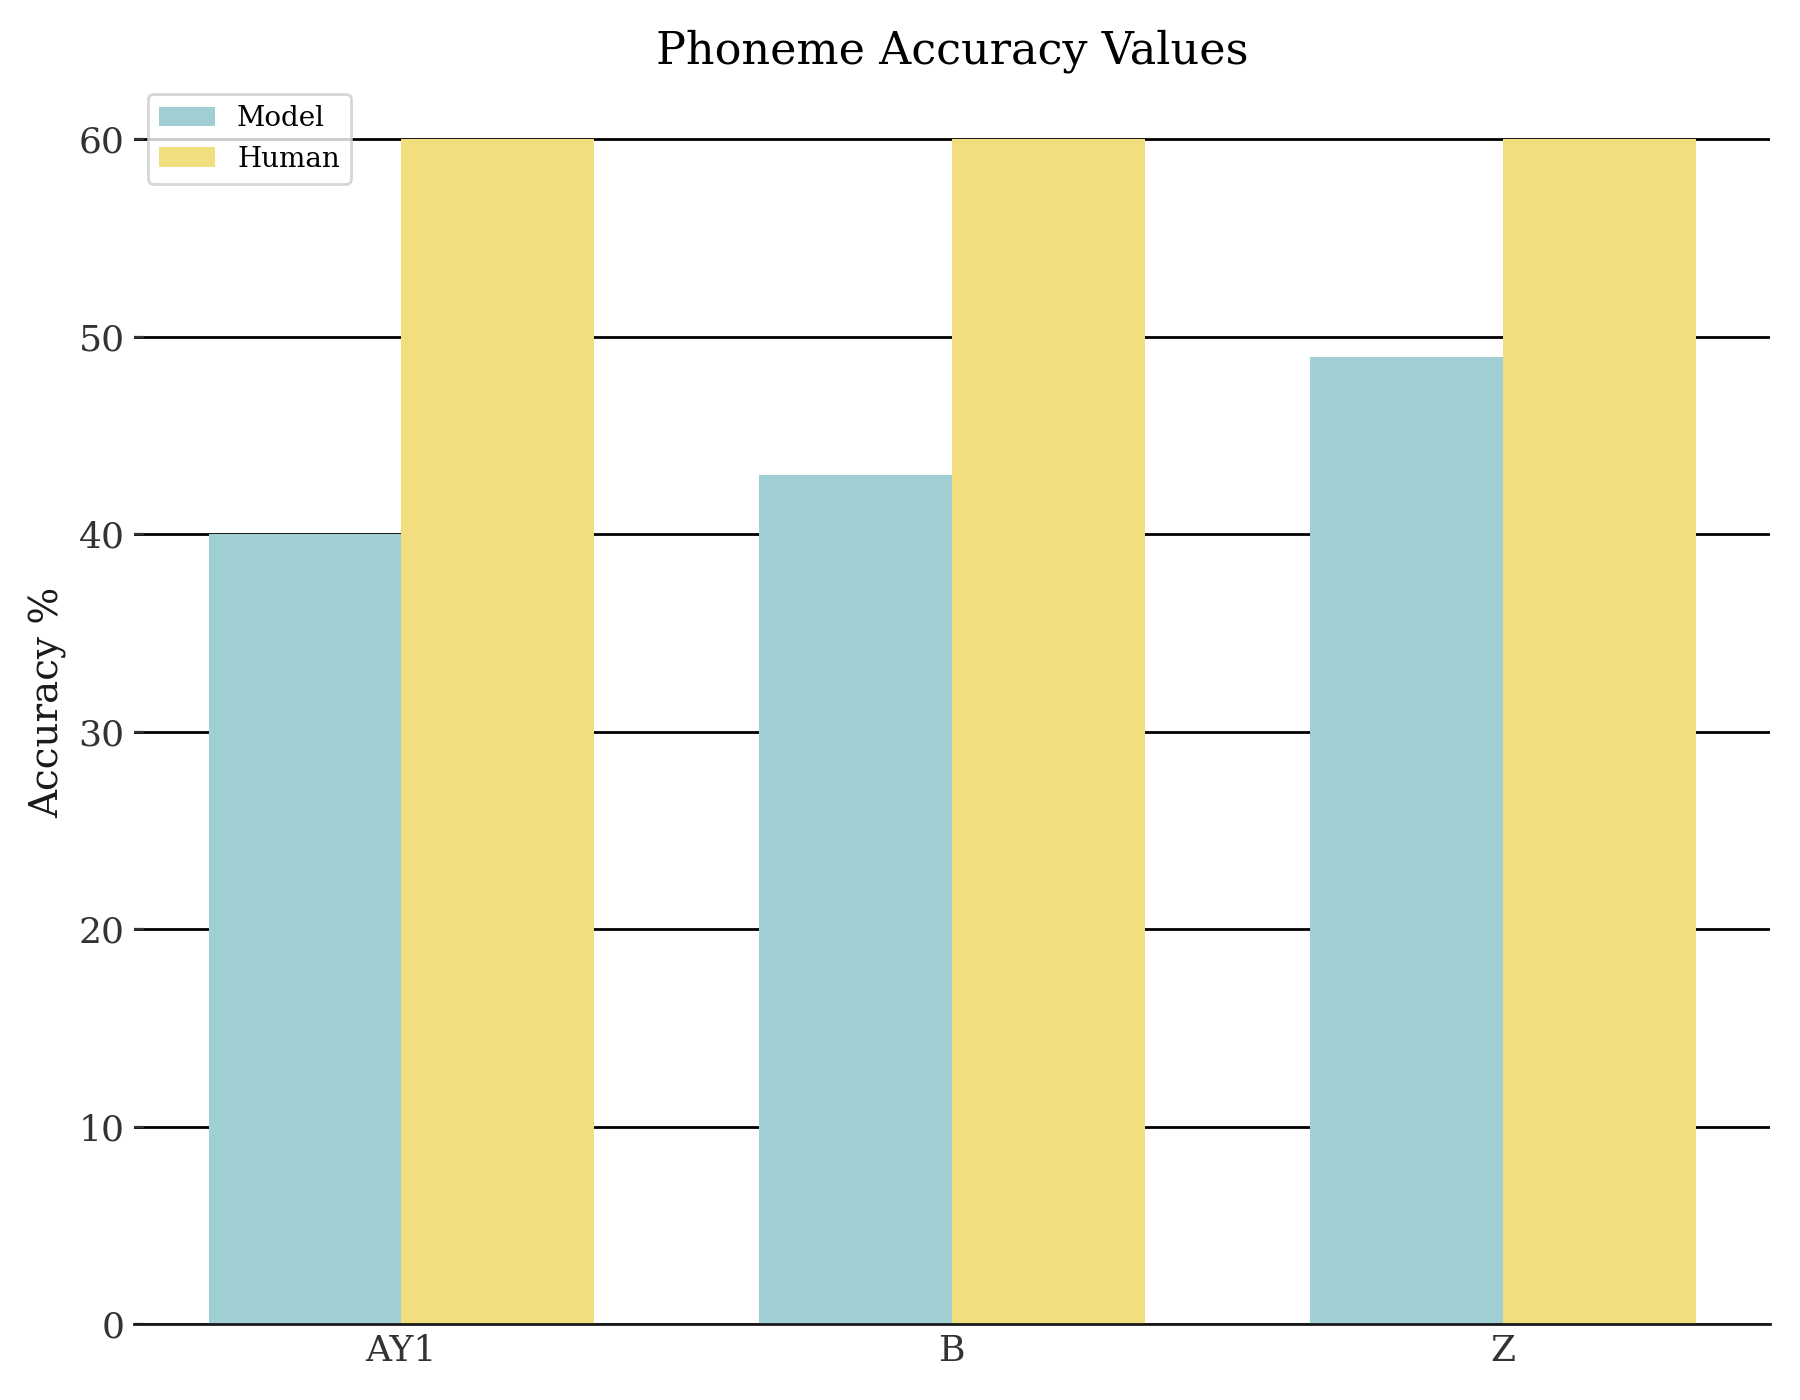
\includegraphics[width=0.65\textwidth]{res/Phone_model_acc.png}
    \caption{A comparison of the accuracies on the individual phonemes from the FER model and human annotators on static images. The latter are better, while also having a consistent accuracy on the phonemes.}
    \label{fig:phone_model_human}
\end{figure}

\subsubsection{Further Evaluation and Validation}
We can further evaluate the annotation accuracy based on the actors and selectors. Figure \ref{fig:actor_overview} shows a consistent annotation accuracy over all four actors. We thus conclude that there was no noticeable bias depending on the actors gender or appearance, and that the annotation difficulty was similar between the two groups.

Figure \ref{fig:selector_overview} presents the individual selectors accuracy on image and video data respectively. With one exception, all annotators performed better on video data. We also see no significant outliers which would indicate random sampling or fraudulent performance by looking up the ground truth labels.

\begin{figure}
    \centering
    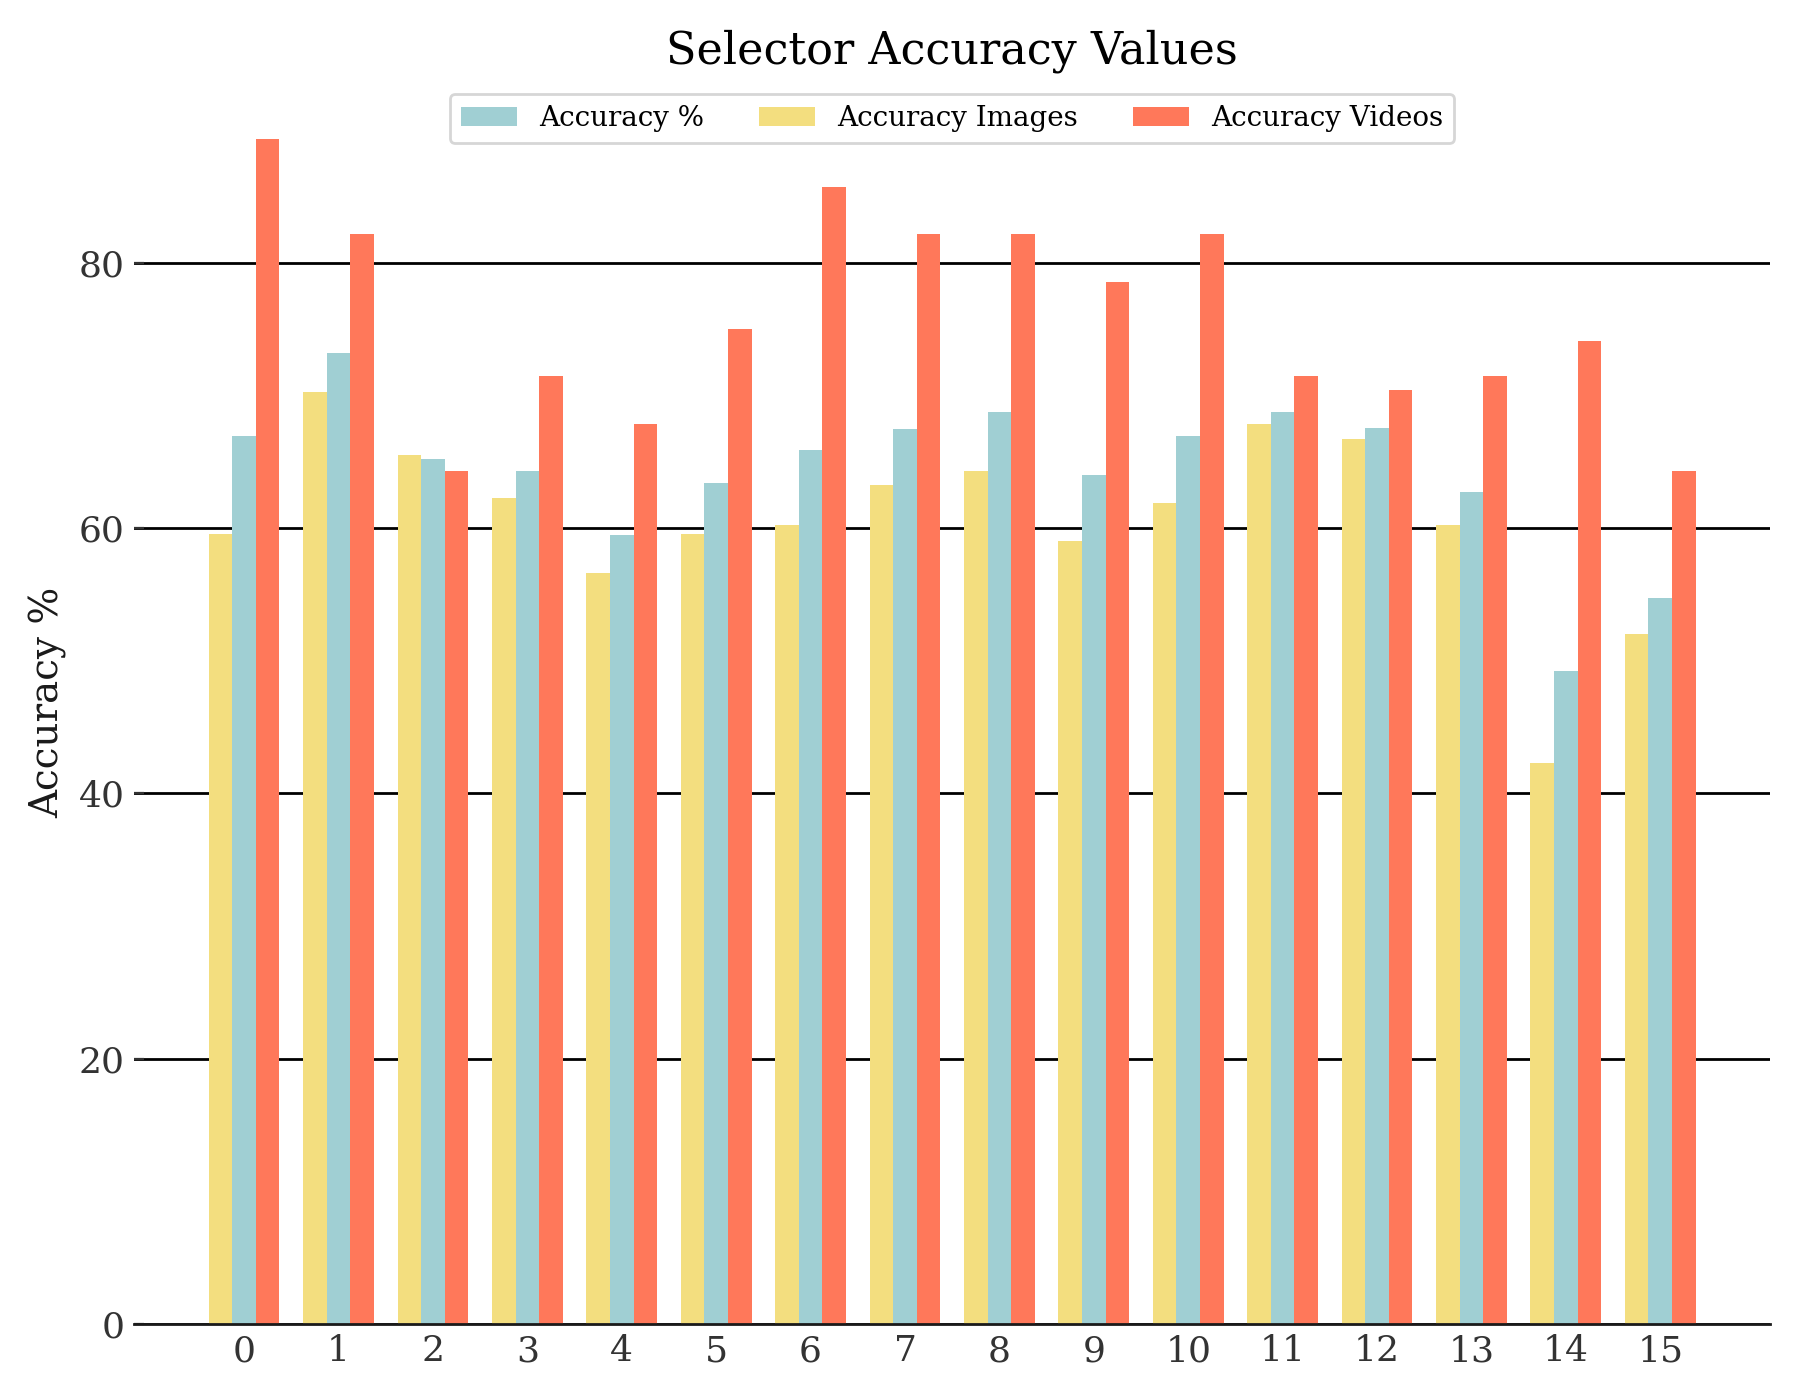
\includegraphics[width=0.75\textwidth]{res/Selector_overview.png}
    \caption{The annotators individual performance. The pattern of videos being labelled more accurately than images is consistent, with one exception on annotator 2.}
    \label{fig:selector_overview}
\end{figure}
\begin{figure}
    \centering
    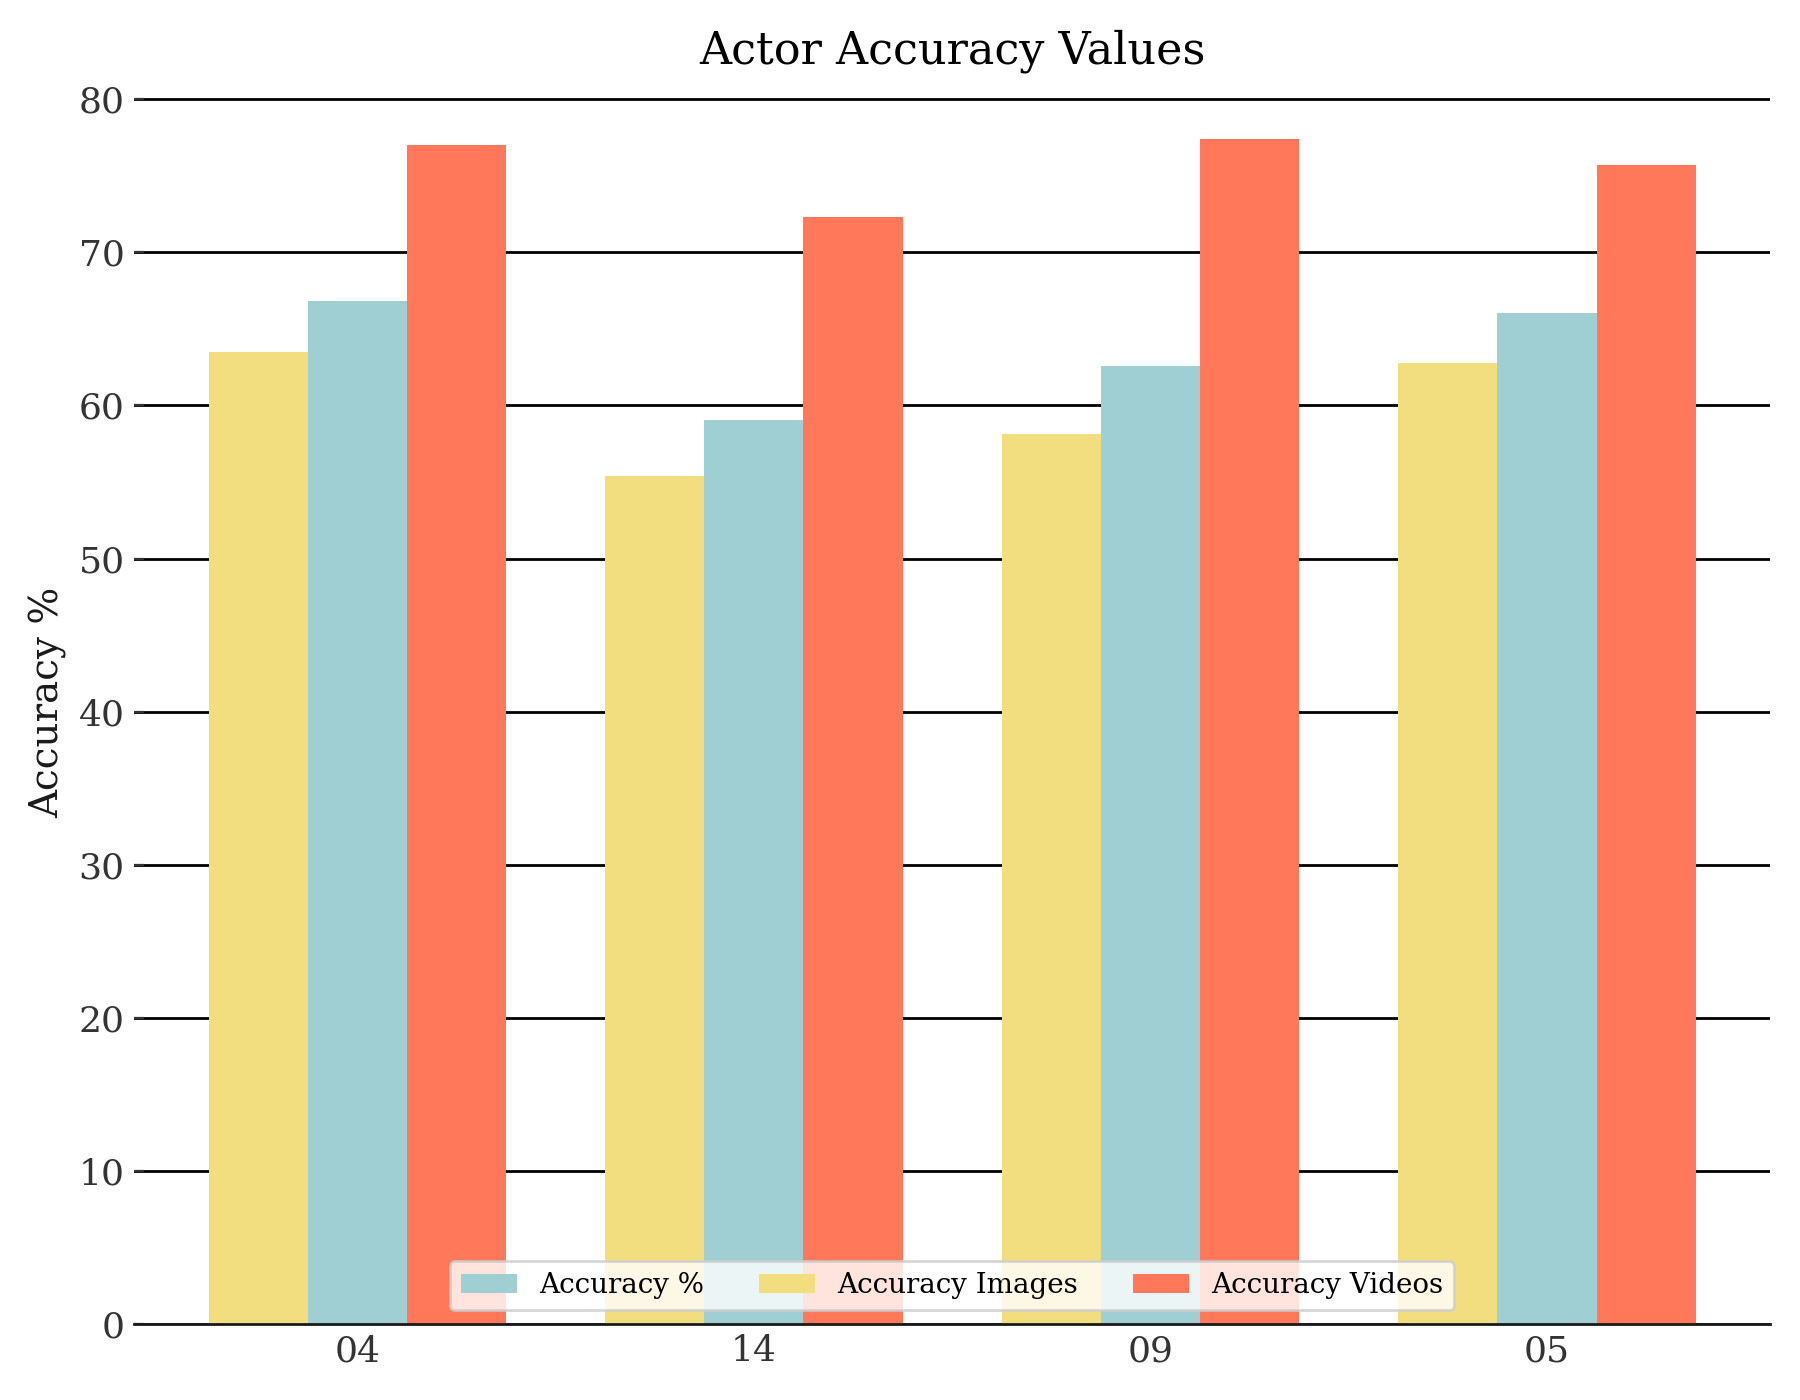
\includegraphics[width=0.75\textwidth]{res/Actor_overview.png}
    \caption{The annotation accuracy depending on the actor. The performance was similar over all actors, concluding that there was no bias depending on appearance or gender.}
    \label{fig:actor_overview}
\end{figure}

The accuracy depending on the presented emotion differs as well. Our annotators were significantly more accurate on videos of an \texttt{angry} emotion, and did do significantly better on \texttt{sad} videos as well. There is also a split in difference between video and image labels depending on the emotion. While \texttt{sad}, \texttt{angry}, and \texttt{fearful} videos were labelled significantly better than their image counterparts, the other emotions had comparable performance. In the case for neutral videos the images were labelled more accurately than the videos.
